%\documentclass{article}
%\documentclass[journal]{IEEEtran}
\documentclass[letterpaper, twoside, openright]{report}
%\documentclass{ActaOulu}
%\documentclass{memoir}

\usepackage{color}
\usepackage{graphicx}
\graphicspath{ {figures/ASUDS_block_diagram(s)_5-2-2015/} }
\usepackage{array}
\usepackage{bigstrut}
\usepackage{authblk}
\usepackage{mathtools}

\usepackage{url}
\usepackage{hyperref}
\hypersetup{colorlinks=true, filecolor=blue, citecolor=red, linkcolor=black, urlcolor=blue}

\begin{document}

\title{Ultrasonics Spectrometer Code Manual}
\author{Matthew Rothfuss\thanks{\href{mailto:mrengr@phys.ksu.edu}{mrengr@phys.ksu.edu}, \href{mailto:mrengr@k-state.edu}{mrengr@k-state.edu}, \href{mailto:rothfuss212@gmail.com}{rothfuss212@gmail.com}}}
\affil{Department of Animal Science and Food Industry, Kansas State University}

\maketitle

%\begin{figure}[h]
%    \centering
%    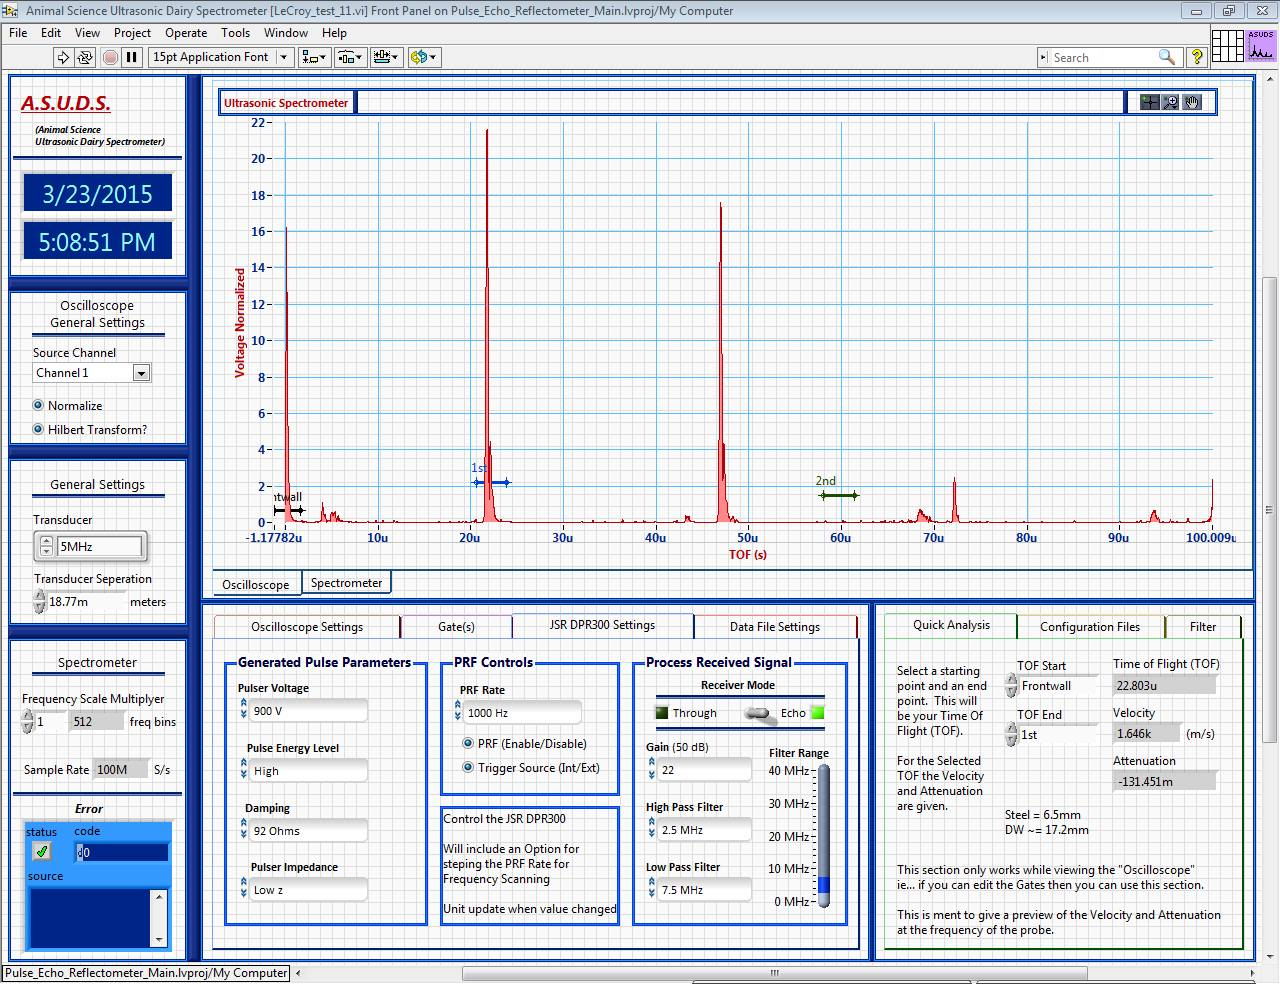
\includegraphics[width=3.0in]{title_page}
%    \caption{Animal Science Ultrasonic Dairy Spectrometer (ASUDS)}
%    \label{Title_Pic}
%\end{figure}

%\begin{abstract}
%Start with an area of civil society where deliberation is occurring (or needs to occur). Identify the barriers to more effective deliberation that are present in this situation and explain them using concepts found in this week's readings. Is there a way for argument/advocacy/debate to address this issue? DO NOT use an example already found in the text or extensively discussed in class---there are plenty of other ones out there for you to choose from.
%\end{abstract}


\tableofcontents


\chapter{LabView Basics}

\section{Introduction}

LabVIEW	(short	for	\textbf{Lab}oratory	\textbf{V}irtual	\textbf{I}nstrumentation	\textbf{E}ngineering	\textbf{W}orkbench) is a development environment for visual programming, developed by National Instruments (\href{http://www.ni.com/}{www.ni.com}). The code files (or program files) are identified by the \textbf{.vi} extension called \textbf{Virtual Instruments} or \textbf{VIs} for short. This graphical language is most commonly used for data acquisition, instrument control, signal processing (analysis), industrial automation, and more.
\\ \\
The next section will cover some basics of LabVIEW design and operation. For additional resources, the current (2013) LabVIEW Getting Started Manual is located \href{http://www.ni.com/pdf/manuals/373427j.pdf}{here}.

\subsection{Additional Resources}

\cite{gomez_alvarez-arenas_air-coupled_2003}

\chapter{Theory of Operation}

Define the background concepts of how/what this program is accomplishing.  Make refs to papers but don't do the math here (don't have time for that).  Just outline the basics of what we want to do, what goes into the system, what the system does (ref manuals and such for theory \& papers), and what the system outputs.
\\ \\

\chapter{Code Structure}

Theory of code operation goes here. ie case structure, state machine, 
\\ \\
\section{Main VI}

Define the outline of the Main VI (the main program) and hit on each part of it.  Don't spend time explaining the subvi's here since i'm doing that in the \textbf{Custom VI's} section. Make sure to to be thorough on all the code that is not included in the subvi section.
\\ \\
The main program \textbf{ASUDS\_v13.vi} is contained within a Project file called \textcolor{red}{(file name here)}.

\section{Custom VI's}

List of custom VI's and a short description of what they do. In the next section we will take a deeper look into each of these subvi's.

\begin{table}
	\centering
	\begin{tabular}{ m{2.5cm} | m{5cm} | m{5cm} }
		\hline
		\hline \multicolumn{3}{c}{Oscilloscope} \\ \hline \hline
		VI & File Name & Description \\ \hline
		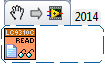
\includegraphics[scale=0.625]{LC931C_Read_main} & LC931C\_Read.vi & Load Oscilloscope Setting from System Generated File \\ \hline
		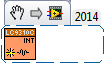
\includegraphics[scale=0.625]{LC931C_Int_main_02} & LC931C\_Int.vi & Initialize Oscilloscope Settings \\ \hline
		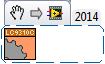
\includegraphics[scale=0.625]{LC931C_settings_main_01} & LC931C\_settings.vi & Apply Settings to Oscilloscope \\ \hline
		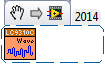
\includegraphics[scale=0.625]{LC931C_single-wave-output_main_01} & LC931C\_single-wave-output.vi & Acquire Single Wave from Oscilloscope and Average \\ \hline
		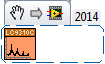
\includegraphics[scale=0.625]{LC931C_norm-pad-hilbert_main_01} & LC931C\_norm-pad-hilbert.vi & Oscilloscope Tab Settings \\ \hline
		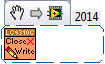
\includegraphics[scale=0.625]{LC931C-Config-Write-Close_main_01} & LC931C-Config-Write-Close.vi & Write Oscilloscope settings to System File and close Oscilloscope resources \\ \hline
	\end{tabular}
	\caption{Oscilloscope Custom VI's}
	\label{tab:1}
\end{table}

\begin{table}
	\centering
	\begin{tabular}{ m{2.5cm} | m{5cm} | m{5cm} }
		\hline
		\hline \multicolumn{3}{c}{JSR Pulser/Receiver} \\ \hline \hline
		VI & File Name & Description \\ \hline
		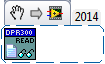
\includegraphics[scale=0.625]{DPR300_Read_main} & DPR300\_Read.vi & Load Pulser/Receiver Setting from System Generated File \\ \hline
		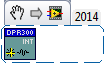
\includegraphics[scale=0.625]{DPR300_Int_main_02} & DPR300\_Int.vi & Initialize Pulser/Receiver Settings \\ \hline
		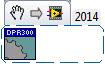
\includegraphics[scale=0.625]{DPR300_settings_main_01} & DPR300\_settings.vi & Apply Settings to Pulser/Receiver \\ \hline
		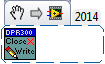
\includegraphics[scale=0.625]{DPR300-Config-Write-Close_main_01} & DPR300-Config-Write-Close.vi & Write Pulser/Receiver settings to System File and close Pulser/Receiver resources \\ \hline
	\end{tabular}
	\caption{JSR Pulser/Receiver Custom VI's}
	\label{tab:2}
\end{table}

\begin{table}
	\centering
	\begin{tabular}{ m{2.5cm} | m{5cm} | m{5cm} }
		\hline
		\hline \multicolumn{3}{c}{Ultrasonic Package} \\ \hline \hline
		VI & File Name & Description \\ \hline
		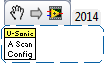
\includegraphics[scale=0.625]{USonic-A-Scan-Config-edit_main_01} & USonic-A-Scan-Config-edit.vi & Configure/Set Gates for Data Acquisition \\ \hline
		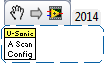
\includegraphics[scale=0.625]{USonic-A-Scan-Config-edit_main_01} & USonic-Gates-edit.vi & Pull Out Relevant Data from Gates for Data Acquisition \\ \hline
		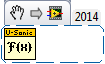
\includegraphics[scale=0.625]{USonic-FFT_main_01} & USonic-FFT.vi & Process Gate For Quick Analysis \\ \hline
	\end{tabular}
	\caption{Ultrasonic A-Scan Customized Package VI's}
	\label{tab:3}
\end{table}

\begin{table}
	\centering
	\begin{tabular}{ m {2.5cm} | m{5cm} | m{5cm} }
		\hline
		\hline \multicolumn{3}{c}{Math} \\ \hline \hline
		VI & File Name & Description \\ \hline
		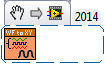
\includegraphics[scale=0.625]{Waveform-to-XY-Array_main_01} & Waveform-to-XY-Array.vi & Convert Waveform to XY-Array \\ \hline
		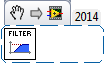
\includegraphics[scale=0.625]{Filter_signal_main_01} & Filter\_signal.vi & Filter Wave Signal for Oscilloscope Tab (does not affect Data Acquisition) \\ \hline
		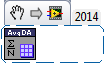
\includegraphics[scale=0.625]{Average-Dynamic-Array_main_01} & Average-Dynamic-Array.vi & Take the Average of N elements in a Dynamic Array \\ \hline
		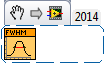
\includegraphics[scale=0.625]{FWHM-Poly_main_01} & FWHM-Poly.vi & Compute the Full Width Half Max (FWHM) of either a Waveform, XY-Graph, or Waveform cluster \\ \hline
		\hline
	\end{tabular}
	\caption{Custom Math VI's}
	\label{tab:4}
\end{table}

\begin{table}
	\centering
	\begin{tabular}{ m {2.5cm} | m{5cm} | m{5cm} }
		\hline
		\hline \multicolumn{3}{c}{Miscellaneous} \\ \hline \hline
		VI & File Name & Description \\ \hline
		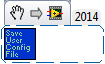
\includegraphics[scale=0.625]{Save-User-Config-File_main_01} & Save-User-Config-File.vi & Save all front panel controls to a user.ini settings file \\ \hline		
		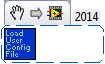
\includegraphics[scale=0.625]{Load-User-Config-File_main_01} & Load-User-Config-File.vi & Load the user.ini settings file \\ \hline
		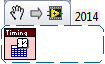
\includegraphics[scale=0.625]{Time-Data_main_01} & Time-Data.vi & Load and Save Data Timing table \\ \hline
		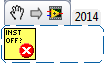
\includegraphics[scale=0.625]{Instrument-error-handler_main_01} & Instrument-error-handler.vi & Pop-up error message for loss of Instrument signal\\ \hline
		\hline
	\end{tabular}
	\caption{Miscellaneous Custom VI's}
	\label{tab:5}
\end{table}

\section{Operation}



\bibliography{ultrasound-ref-01}
\bibliographystyle{unsrt}

\end{document}
